\begin{frame}
    \frametitle{前情回顾}
    \begin{itemize}
        \item 量子化光场~~真空态~~产生湮灭算符 
        \item 相干态~~ 平移算符 ~~相图
        \item 压缩态~~ 压缩算符
        \item 数态表象~~数态展开
        \item 参量下转换~~平衡零差探测 
        \item 光子计数 ~~ 亚泊松~~泊松~~超泊松光场 
    \end{itemize}     
\end{frame}

%%%%%%%%%%%%%%%%%%%%%%%%%%%%%%%%%%
\begin{frame} [plain]
    \frametitle{}
    \Background[1] 
    \begin{center}
    {\huge 第11-12讲:场关联函数}
    \end{center}  
    \addtocounter{framenumber}{-1}   
\end{frame}

\section{1. 星光测量HB-T 实验}

\begin{frame} 
 \frametitle{实验原理}
 汉伯里·布朗(Hanbury Brown)和特维斯(Twiss)是天文学家,他们想通过星光测量恒星的直径.
 为此他们革新了迈克耳逊恒星干涉仪.
   \begin{center}
        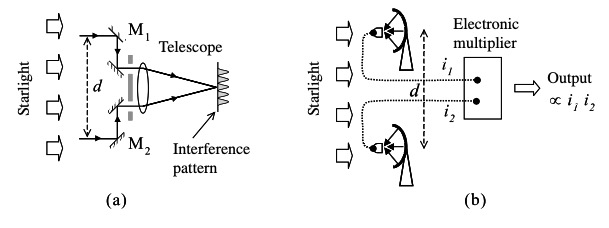
\includegraphics[width=1.0\textwidth]{figs/2022-05-08-12-30-39.png}
   \end{center}
\end{frame}

\begin{frame}
 \frametitle{}
 迈克耳逊恒星干涉仪: 点光源的光是相干光, 平行光是相干光, 小角度的非平行光是部分相干光. \\ 
 由于地球与恒星的距离(L)远大于恒星的直径(D), 可以满足小角度条件.
 \[ \delta \theta_s =\frac{D}{L}\] 
 由于时间和空间相干性的限制, 迈克耳逊恒星干涉仪存在极限:
 \[ \delta \theta_r\leq 1.22 \frac{\lambda}{d}\] 
 当 $d> 1.22 \lambda /\delta \theta_s$, 则没有干涉条纹.  \\ 
 因此, 把d从小依次变大, 会出现在某个d时,干涉条纹刚好消失, 由此可得到$\theta_s$, 进而得到恒星的直径D. 
\end{frame}

\begin{frame} 
 \frametitle{}
 但是$d$增大时,保持两收集镜片的稳定性会变得越来越困难(不稳定性会导致角度误差变大). 因此, 迈克耳逊恒星干涉仪不能用来测量很大的恒星. \\ {\vspace*{2.3em}}
 计算迈克耳逊恒星干涉仪的光强
 \[ \begin{aligned}
     E&= E_k (e^{\mathbf{ik}\cdot \mathbf{r}_1}+ e^{\mathbf{ik}\cdot \mathbf{r}_2}) + E_{k'} (e^{\mathbf{ik'}\cdot \mathbf{r}_1}+ e^{\mathbf{ik'}\cdot \mathbf{r}_2}) \\ 
     I&= \kappa \left\langle E^* E \right\rangle \\
     &= \kappa \left\langle 2 \left| E_k\right|^2 + 2\left| E_{k'}\right|^2 + \left|E_k\right|^2 (e ^{i \mathbf{k}\cdot(\mathbf{r}_1-\mathbf{r}_2)+c.c.})  \right\rangle \\
 \end{aligned}\]
\end{frame}

\begin{frame} 
\frametitle{}
 取 $\left| E_{k}\right|^2 \approx \left| E_{k'}\right|^2 = I_0$, $\mathbf{r}_0 = \dfrac{\mathbf{r}_1 - \mathbf{r}_2}{2}$    
 光强为
 \[ I = 4 \kappa I_0 \left\{ 1+\cos\left[ (\mathbf{k} + \mathbf{k}')\cdot \mathbf{r}_0\right] \cos\left( (\mathbf{k} - \mathbf{k}')\cdot \mathbf{r}_0 \right)  \right\}\]
分析: \\ 
 (1) $\mathbf{k} - \mathbf{k}'$大气的扰动相互抵消, 因此, 调节位置, 可使 \[\cos\left( (\mathbf{k} - \mathbf{k}')\cdot \mathbf{r}_0 \right)=1 \]
(2) 问题在
\[ \cos\left[ (\mathbf{k} + \mathbf{k}') \cdot \mathbf{r}_0 \right] \]
没有办法处理. 而这是一个变化很快的敏感项, 大气的扰动和仪器的噪声涨落可导致其平均值归零, 从而限制了迈克耳逊恒星干涉仪的使用 
\end{frame}

\begin{frame} 
\frametitle{}
 汉伯里·布朗(Hanbury Brown)和特维斯(Twiss) 在1954-1957年间,提出可HB-T实验来测量恒星的直径. \\
 革新点:
 \begin{enumerate}
     \item 改平面镜为凹面镱, 可以收集更多的光, 可测量暗些的恒星
     \item 改相位干涉(关联)为强度干涉(关联)
 \end{enumerate}
 HB-T实验是整个量子光学的奠基性实验!
\end{frame}

\begin{frame} 
 \frametitle{}
    现在要证明两光场的强度之间存在关联!   
    \begin{center}
        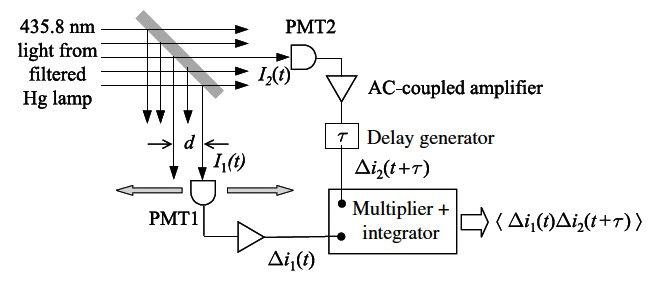
\includegraphics[width=0.6\textwidth]{figs/2022-05-08-13-20-54.png}
   \end{center}
   量子力学中,如果两函数不正交(内积不为零),则它们线性相关, 是有关联的.
   \[ \int \psi^*_1(\mathbf{r_1},t) \psi_2(\mathbf{r_2},t+ \tau) \mathbf{dr}dt \not = 0 \]
因此, HB-T 实验本质上是两光场波函数的内积不为零的问题.
\end{frame}

\section{2. 半经典关联函数}

 \begin{frame} 
  \frametitle{一阶关联函数}
  根据半经典测量理论,若光场强度函数为$I(\mathbf{r},t)$ , 则在  $ \Delta t $ 时间内,测到发生光电发射事件的差分概率为 
\[  P (\mathbf{r},t) \Delta t = \eta \left\langle I(\mathbf{r},t) \right\rangle \Delta t \]  
代入电场强度, 有:   
\[ \begin{aligned}
    P (\mathbf{r},t) \Delta t &= \eta \left\langle I(\mathbf{r},t) \right\rangle \Delta t \\ 
    & = \eta \left\langle E^* (\mathbf{r},t) E (\mathbf{r},t)\right\rangle \Delta t \\
    &=\eta G^{1} (\mathbf{r},t) \Delta t  \\
\end{aligned}\] 
 \end{frame}

 \begin{frame} 
  \frametitle{}
  上式中,定义了内积函数:
\[ \boxed{ G^{(1)} (\mathbf{r},t) = \left\langle E^* (\mathbf{r},t) E (\mathbf{r},t)\right\rangle} = \int E^* (\mathbf{r},t) E (\mathbf{r},t) d \mathbf{r} dt \]
  称为一阶关联函数, 它描述了光场的自相关性.\\ 
  \[ \begin{aligned}
    P (\mathbf{r},t) \Delta t &=\eta G^{1} (\mathbf{r},t) \Delta t  \\
   \end{aligned}\] 
   表明: 测量发生光电发射事件的概率,用一阶关联函数描述. 
 \end{frame}

 \begin{frame}   
    \frametitle{二阶关联函数}
   如果有两个探测器, 则
    \[ \begin{aligned}
      P (\mathbf{r_1},t_1) \Delta t_1 &=\eta \left\langle E^*_1 (\mathbf{r_1},t_1) E_1 (\mathbf{r_1},t_1)\right\rangle \Delta t_1  \\
      P (\mathbf{r_2},t_2) \Delta t_2 &=\eta \left\langle E^*_2 (\mathbf{r_2},t_2) E_2 (\mathbf{r_2},t_2)\right\rangle  \Delta t_2  \\
     \end{aligned}\] 
    两探测器相互独立, 则两探测器都测得发生光电发射事件的概率为 (没有归一化):
    \[ \begin{aligned}
        P_2 (\mathbf{r_1},t_1; \mathbf{r_2},t_2)  &= P (\mathbf{r_1},t_1) \Delta t_1 P (\mathbf{r_2},t_2) \Delta t_2\\
        &= \eta_1 \eta_2 \left\langle E^*_1 (\mathbf{r_1},t_1) E_1 (\mathbf{r_1},t_1)\right\rangle  \left\langle E^*_2 (\mathbf{r_2},t_2) E_2 (\mathbf{r_2},t_2)\right\rangle \Delta t_1 \Delta t_2 \\
    \end{aligned}\] 
    如果两探测器相互不独立, 则:
    \[ \begin{aligned}
        P_2 (\mathbf{r_1},t_1; \mathbf{r_2},t_2)  
        &= \eta_1 \eta_2 \left\langle E^*_1 (\mathbf{r_1},t_1) E_1 (\mathbf{r_1},t_1) E^*_2 (\mathbf{r_2},t_2) E_2 (\mathbf{r_2},t_2)\right\rangle \Delta t_1 \Delta t_2 \\
        &= \eta_1 \eta_2  G^{(2)} (\mathbf{r_1},t_1; \mathbf{r_2},t_2) \Delta t_1 \Delta t_2 
    \end{aligned}\]
\end{frame}

\begin{frame} 
 \frametitle{}
 上式中,定义了函数:
 \[ \boxed{ \begin{aligned}   
 G^{(2)} (\mathbf{r_1},t_1; \mathbf{r_2},t_2)  &= \left\langle E^*_1 (\mathbf{r_1},t_1) E_1 (\mathbf{r_1},t_1) E^*_2 (\mathbf{r_2},t_2) E_{2} (\mathbf{r_2},t_2)\right\rangle \\ 
 &= \left\langle I_1 (\mathbf{r_1},t_1) I_2 (\mathbf{r_2},t_2)\right\rangle
\end{aligned}} \]
称为二阶关联函数, 它描述了两光场强度之间的相关性. 或者说两个探测器测得的光场强度的相关性. \\ 
如果只考虑时间关联, 则描述同一电场不同时刻相关性的函数为:
\[ \begin{aligned}
    G^{(2)}(\tau) &= G^{(2)}(t; t+ \tau) \\
    &= \left\langle E^* (t) E (t) E^* (t+ \tau) E (t+ \tau)\right\rangle \\
    &= \left\langle I (t)  I (t+ \tau)\right\rangle \\ 
\end{aligned}\] 
\end{frame}

\begin{frame}
\frametitle{}
 归一化的场关联函数为:
\[  g^{(1)} (\mathbf{r},t) =  \frac{\left\langle E^* (\mathbf{r},t) E (\mathbf{r},t)\right\rangle} {\left\langle E^* (\mathbf{r},t)\right\rangle\left\langle E (\mathbf{r},t)\right\rangle}  \]
\[ \begin{aligned}   
    g^{(2)} (\mathbf{r_1},t_1; \mathbf{r_2},t_2)  
    &= \frac{\left\langle I_1 (\mathbf{r_1},t_1) I_2 (\mathbf{r_2},t_2)\right\rangle}{\left\langle I_1 (\mathbf{r_1},t_1)\right\rangle\left\langle I_2 (\mathbf{r_2},t_2)\right\rangle}
   \end{aligned} \]
\end{frame}

 \begin{frame} 
  \frametitle{分析}
  同一时刻的相关性
  \[  g^{(2)}(0) = \frac{\left\langle I (t)  I (t+ \tau)\right\rangle} {\left\langle I (t) \right\rangle \left\langle I (t+ \tau)\right\rangle} =  \frac{\left\langle I^2 (t)  \right\rangle}{\left\langle I (t)\right\rangle^2 }  \geq 1\]
  对于相干态, $  \left\langle I^2 (t)  \right\rangle = \left\langle I (t) \right\rangle^2, \quad g^{(2)}(0) =1 $ \\ 
  对于混沌光束, $ \left\langle I^2 (t)  \right\rangle > \left\langle I(t) \right\rangle^2, \quad g^{(2)}(0) >1 $
\end{frame}

\begin{frame} 
      \frametitle{}   
  设光束的相干时间为$\tau_c$ (原子能级的寿命),当$\tau\gg \tau_c$, 没有时间相干性, 则 
  \[ I (t) = \left\langle I \right\rangle  + \Delta I (t) =  \left\langle I  \right\rangle  \] 
  \[ \begin{aligned}
    g^{(2)}(\tau) &= \frac{\left\langle I (t)  I (t+ \tau)\right\rangle }{\left\langle I (t) \right\rangle \left\langle  I (t+ \tau)\right\rangle }\\ 
    &= \frac{\left\langle \left\langle I  \right\rangle  \left\langle I  \right\rangle \right\rangle}{\left\langle I \right\rangle^2} \\
    &= 1 
\end{aligned}\]     
\end{frame}
  
 \begin{frame} 
  \frametitle{}
      对于相干态, 恒有 $ I (t)= I (0) =I$ 
      \[ \begin{aligned}
        g^{(2)}(\tau) &= \frac{\left\langle I (t)  I (t+ \tau)\right\rangle}{\left\langle I (t) \right\rangle \left\langle I (t+ \tau)\right\rangle} \\ 
        &= \frac{\left\langle I^2\right\rangle}{ \left\langle I\right\rangle ^2} \\
        &= 1   
    \end{aligned}\] 
      \begin{center}
           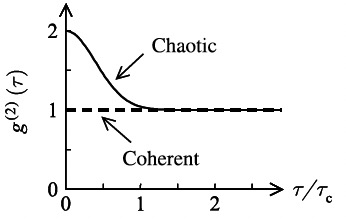
\includegraphics[width=0.5\textwidth]{figs/2022-05-08-15-34-39.png}
      \end{center} 
    * 半经典二阶关联函数只能描述经典光和相干光的光强相关性,不能给出非经典光的物理图像.
 \end{frame}

 \begin{frame} 
  \frametitle{}
  热辐射光场的一阶关联函数:
  \[ g^{(1)}(\tau) = \frac{\sum_k \overline{n}_k \omega_k \exp{(-i \omega_k \tau)} }{\sum_k \overline{n}_k \omega_k}, \quad g^{(2)}(\tau) =1+ \left|g^{(1)}(\tau) \right|^2\]
  对于高斯混沌光束: 
       \[g^{(2)}(\tau) =1 + e^{-\pi (\frac{\tau}{\tau_c})^2 } \]
  对于洛伦兹混沌光束
       \[g^{(2)}(\tau) =1 + e^{-2 \frac{\left|\tau\right|}{\tau_0} } \]
         \begin{center}
              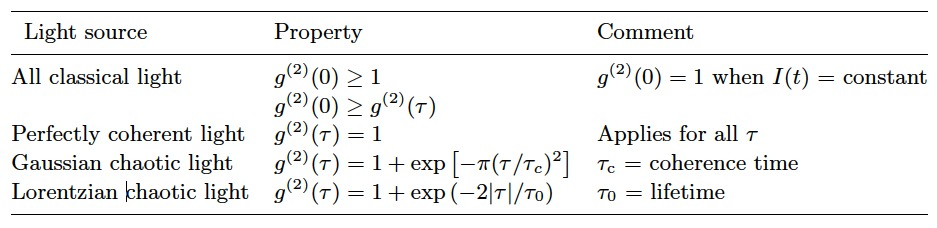
\includegraphics[width=1.0\textwidth]{figs/2022-05-08-16-01-24.png}
         \end{center}
 \end{frame}

\section{3. 量子关联函数}

 \begin{frame} 
  \frametitle{ 光子HB-T实验}
         \begin{center}
              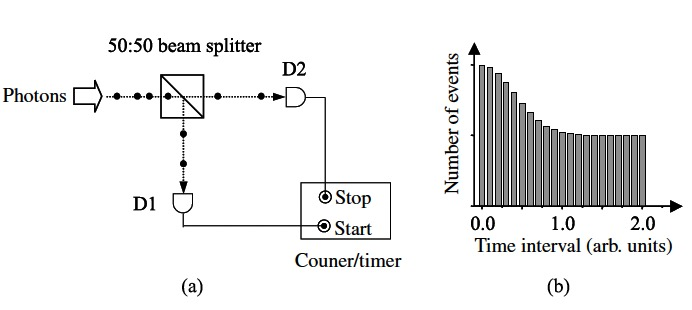
\includegraphics[width=0.8\textwidth]{figs/2022-05-08-16-13-39.png}
         \end{center}
     如光强很弱, 则要使用单光子探测器进行计数, 那两计数之间是否存在关联?
 \end{frame}

 \begin{frame} 
    \frametitle{}
    平稳随机过程假设\\
    (1) 统计的稳定性(statistically stationary)\\ 
    对任意时间$T$,下面的联合测量概率恒成立.
         \[ P_{n}\left(x_{n}, t_{n} ; x_{n-1}, t_{n-1} ; \ldots ; x_{1}, t_{1}\right)=P_{n}\left(x_{n}, t_{n}+T ; x_{n-1}, t_{n-1}+T ; \ldots ; x_{1}, t_{1}+T\right)\]
    (2) 性质: \\ 
    时间原点选取不影响概率
    \[ P_1(x,t)=P_1(x,0)\]
    对空间的概率积分不依赖于时间原点选取
    \[ \left\langle x(t) \right\rangle = \int x P_1(x,t)dx=  \int x P_1(x,0)dx  \]
    \end{frame}

 \begin{frame} 
  \frametitle{}
    分析: 单光子探测器, 测得的光子数(计数)服从泊松分布(平稳随机过程)
       \[  P_n = \frac{\overline{n}^n }{n!} \mathrm{e}^{- \overline{n} }\]
       计数均值:
    \[ \begin{aligned}
        \overline{n} &= \sum_n n P_n\\
        &=\sum_n n \frac{\overline{n}^n }{n!} \mathrm{e}^{- \overline{n} } \\
        &= \left\langle \sum_n n \frac{(\eta I)^n }{n!} \mathrm{e}^{- \eta I }  \right\rangle \\ 
        &= \left\langle (\eta I) \frac{\mathrm{d}}{\mathrm{d}(\eta I)}\sum_n  \frac{(\eta I)^n }{n!} \mathrm{e}^{-\eta I }  \right\rangle \\
        &=  \left\langle \eta I \right\rangle = \eta \left\langle I \right\rangle
    \end{aligned}\] 
 \end{frame}

 %\begin{frame} 
 % \frametitle{}
 % 平方数均值:
 % \[ \begin{aligned}
 %   \overline{n^2} &= \sum_n n^2 P_n\\
 %   &= \sum_n n(n-1) P_n +\sum_n n  P_n \\ 
 %   &= \eta \left\langle I \right\rangle + \eta^2 \left\langle I^2 \right\rangle 
 %   \end{aligned}\] 
 %   均方差:
 %   \[ \begin{aligned}
 %       \left\langle (\Delta n)^2 \right\rangle &= \overline{n^2} -\overline{n}^2 \\ 
 %       &= \overline{n} + \eta^2 \left\langle I^2 \right\rangle 
 %   \end{aligned}\]     
 %\end{frame}

 \begin{frame}  
  \frametitle{}
      若两探测器量子效率相同,根据二阶关联函数的定义, 有:
      \[ \begin{aligned}
        g^{(2)}(\tau) &= \frac{\left\langle I_1 (t)  I_2 (t+ \tau)\right\rangle }{\left\langle I_1 (t) \right\rangle  \left\langle I_2 (t+ \tau)\right\rangle }\\ 
        &=  \frac{\left\langle n_1 (t)  n_2 (t+ \tau)\right\rangle}{\left\langle n_1 (t)\right\rangle \left\langle n_2 (t+ \tau)\right\rangle}
    \end{aligned}\] 
    ~\\ {\vspace*{2.3em}} 
    * 计数相关体现光强相关, 必须采用全量子理论进一步处理.
 \end{frame}

 \begin{frame} 
  \frametitle{}
       {\Bullet}考虑理想光子计数器. 它在时空点$(\mathbf{r}, t)$处吸收了一个光子(即探测到一个光子), 导致场从初态$\rs{i }$ 跃迁到末态$\rs{f}$. \\
       光场可表示为正频部分和负频部分:
       \[ \hat{E} = \hat{E}^{(+)} + \hat{E}^{(-)} =\sum_j \epsilon_j a_j e^{-i(v_j t - \mathbf{k}\cdot \mathbf{r})} + \sum_j \epsilon_j a^{\dagger} _j e^{i(v_j t - \mathbf{k}\cdot \mathbf{r})}\]
       正频是湮灭算符随时间振荡的总和, 与光子被吸收(湮灭)有关,\\ 
       探测概率等于跃迁概率:
       \[T_{if} = \left| \lcr{f}{E^{(+)}(\mathbf{r}, t)}{i} \right|^2\] 
       总探测概率是对所有可能末态求和
       \[ \begin{aligned}
           \omega'_1(\mathbf{r}, t) = \sum_f T_{if} &= \sum_f \left| \lcr{f}{E^{(+)}(\mathbf{r}, t)}{i} \right|^2 \\ 
           &= \sum_f \lcr{i}{E^{(-)}(\mathbf{r}, t)}{f} \lcr{f}{E^{(+)}(\mathbf{r}, t)}{i}   \\
           &= \lcr{i}{E^{(-)}(\mathbf{r}, t)E^{(+)}(\mathbf{r}, t)}{i}  
       \end{aligned}\] 
 \end{frame}

 \begin{frame} 
  \frametitle{}
       若初态是真空态:
       \[ \rho = \rl{0 }{0 }\]
       \[\omega'_1(\mathbf{r}, t)= \lcr{0}{E^{(-)}(\mathbf{r}, t)E^{(+)}(\mathbf{r}, t)}{0} =0 \]
       表示对真空态,探测到一个光子的概率为零. \\ 
      通常,得考虑初态是叠加态$\rs{\psi} = \sum_i a_i\rs{i}$, 或混态, 其密度算符分别为
       \[\rho = \rl{\psi}{\psi} = \sum_i a^*_i a_i\rl{i}{i}; \quad \rho = \sum_n P_n\rl{\psi_n}{\psi_n} = \sum_{n,i} P_n a^*_i a_i\rl{i}{i};  \]
       对应的概率为:
    \[\begin{aligned}
        \omega_1(\mathbf{r}, t)
        &= \sum_i \lcr{i}{a^* _i E^{(-)}(\mathbf{r}, t)E^{(+)}(\mathbf{r}, t) a_i}{i} \\ 
        &= \sum_i a^*_i a_i\rl{i}{i}{E^{(-)}(\mathbf{r}, t)E^{(+)}(\mathbf{r}, t)} \\ 
        &= Tr( \rho E^{(-)}(\mathbf{r}, t)E^{(+)}(\mathbf{r}, t))
    \end{aligned} \] 
 \end{frame}

\begin{frame} 
    \frametitle{}
    基于$\omega_1(\mathbf{r}, t)$, 定义一阶关联函数:
    \[ G^{(1)}(\mathbf{r_1}, \mathbf{r_2},; t_1, t_2) = Tr( \rho E^{(-)}(\mathbf{r_1}, t_1)E^{(+)}(\mathbf{r_2}, t_2)) \]   
    使用记号 $x_i= (\mathbf{r}_i, t_i)$,简写为:
    \[ G^{(1)}(x_1; x_2) = Tr( \rho E^{(-)}(x_1)E^{(+)}(x_2)) \]  
    令$\mathbf{r_1}=\mathbf{r_2}=r,t_1=t, t_2=t+\tau$, 
    \[ G^{(1)}(\mathbf{r} ;t, t+\tau) = Tr( \rho E^{(-)}(\mathbf{r}, t)E^{(+)}(\mathbf{r}, t+\tau)) \] 
    令$\mathbf{r_1}=\mathbf{r_2}=r,t_1=t_2=t$, 退化为测得一个光子的概率
    \[ G^{(1)}(\mathbf{r}, t) = Tr( \rho E^{(-)}(\mathbf{r}, t)E^{(+)}(\mathbf{r}, t))=\omega_1(\mathbf{r}, t) \] 
    很明显, 一阶关联函数描述各种时位条件下测得一个光子事件的概率
   \end{frame}

   \begin{frame} 
    \frametitle{}
    {\Bullet}考虑有两个探测器,在两个不同时-位点各探测到一个光子,则两事件的联合概率为
    \[ \begin{aligned}
        \omega'_2(\mathbf{r_1}, t_1;\mathbf{r_2}, t_2) &= \sum_f \left| \lcr{f}{E^{(+)}(\mathbf{r_1}, t_1)E^{(+)}(\mathbf{r_2}, t_2)}{i} \right|^2 \\ 
        &= \lcr{i}{E^{(-)}(\mathbf{r_1}, t_1)E^{(-)}(\mathbf{r_2}, t_2)E^{(+)}(\mathbf{r_1}, t_1)E^{(+)}(\mathbf{r_2}, t_2)}{i} \\ 
        \omega_2(\mathbf{r_1}, t_1;\mathbf{r_2}, t_2)&=  Tr(\rho E^{(-)}(\mathbf{r_1}, t_1)E^{(-)}(\mathbf{r_2}, t_2)E^{(+)}(\mathbf{r_1}, t_1)E^{(+)}(\mathbf{r_2}, t_2) )
    \end{aligned}\] 
    可定义二阶关联函数:\\ 
    $~ {\hspace*{2em}} G^{(2)}(\mathbf{r_1}, \mathbf{r_2}, \mathbf{r_3}, \mathbf{r_4}; t_1, t_2, t_3, t_4) = $ \[ ~ {\hspace*{3em}} Tr(\rho E^{(-)}(\mathbf{r_1}, t_1)E^{(-)}(\mathbf{r_2}, t_2)E^{(+)}(\mathbf{r_3}, t_3)E^{(+)}(\mathbf{r_4}, t_4) ) \]
    使用记号 $x_i= (\mathbf{r}_i, t_i)$, 简写为:
    \[ G^{(2)}(x_1, x_2; x_3,x_4) = Tr(\rho E^{(-)}(x_1)E^{(-)}(x_2)E^{(+)}(x_3)E^{(+)}(x_4)) \]
\end{frame}

\begin{frame} 
      \frametitle{}
      {\Bullet} 描述$n$个探测器,则使用$n$阶关联函数, 定义为:\\ 
        $~ {\hspace*{2em}} G^{(n)}(x_1,x_2,\cdots, x_n;x_{n+1},\cdots, x_{2n})= $ 
        \[ Tr(\rho E^{(-)}(x_1)E^{(-)}(x_2)\cdots E^{(-)}(x_n) E^{(+)}(x_1)\cdots E^{(+)}(x_n)) \]
        若令 $\tau = t_2-t_1$
    \[\begin{aligned}
        G^{(1)}(\mathbf{r_1}, \mathbf{r_2},; t_1, t_2) &= G^{(1)}(\mathbf{r_1}, \mathbf{r_2},; \tau) \\ 
        &= Tr( \rho E^{(-)}(\mathbf{r_1})E^{(+)}(\mathbf{r_2}, \tau)) 
    \end{aligned} \]
    若令 $\tau_1 = t_3-t_1; \tau_2 = t_4-t_2$ \\
    \[\begin{aligned}
    G^{(2)}(\mathbf{r_1}, \mathbf{r_2}, \mathbf{r_3}, \mathbf{r_4}; & t_1, t_2, t_3, t_4) \\ 
    &= G^{(2)}(\mathbf{r_1}, \mathbf{r_2}, \mathbf{r_3}, \mathbf{r_4};\tau_1,\tau_2 )  \\
    &=  Tr(\rho E^{(-)}(\mathbf{r_1})E^{(-)}(\mathbf{r_2})E^{(+)}(\mathbf{r_3}, \tau_1)E^{(+)}(\mathbf{r_4}, \tau_2) ) 
   \end{aligned} \]
   \end{frame}

   \begin{frame} 
    \frametitle{}
    归一化的场关联函数:
        \[g^{(1)} (x_1,x_2)= \frac{G^{(1)}(x_1; x_2) }{[G^{(1)}(x_1) G^{(1)}(x_2)]^{1/2} }\]
        \[g^{(2)} (x_1, x_2; x_3,x_4)= \frac{G^{(2)}(x_1,x_2; x_3, x_4) }{[G^{(1)}(x_1) G^{(1)}(x_2)G^{(1)}(x_3) G^{(1)}(x_4)]^{1/2} }\]
    ~\\ {\vspace*{1.3em}}
   * 一阶关联函数是一个探测器测得一个光子的概率\\ 
   * 二阶关联函数是二个探测器各测得一个光子的联合概率 \\ 
   * $n$阶关联函数是n个探测器各测得一个光子的联合概率 
   \end{frame}
\begin{frame} [label=current] 
\frametitle{}
    关联函数的产生湮灭算符表示 (平稳随机过程假设)
    \[ \begin{aligned}
        g^{(2)}(\tau) 
        &=  \frac{\left\langle n_1 (t)  n_2 (t+ \tau)\right\rangle}{\left\langle n_1 (t)\right\rangle \left\langle n_2 (t+ \tau)\right\rangle} \\ 
        &=  \frac{\left\langle a^{\dagger} (t)  a^{\dagger} (t+ \tau)\right\rangle}{\left\langle a^{\dagger} a \right\rangle ^2} \\
        g^{(1)}(\tau) &=  \frac{\left\langle a^{\dagger} (t)  a (t+ \tau)\right\rangle}{\left\langle a^{\dagger} a \right\rangle } \\
    \end{aligned}\] 
\end{frame}

\section{4. 应用实例~~反聚束}

   \begin{frame} 
    \frametitle{单光子干涉}
        单光子干涉实验是延迟选择实验的简化版\\ 
        装置如下.
          \begin{center}
               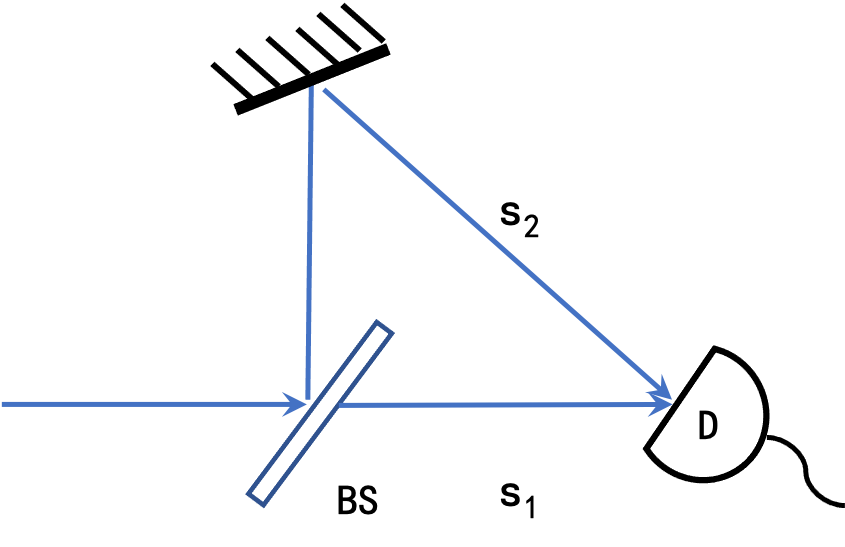
\includegraphics[width=0.4\textwidth]{figs/19.png}
          \end{center}
        实验现象: 通过改变光程差,可有效控制光子计数.
   \end{frame}

   \begin{frame} 
    \frametitle{}
    分析: \\ 
    (1) 这是单光子单模场, 分束器在$t$时刻对光子做第一次测量, 关联函数为:
    \[ \begin{aligned}
        g^{(1)} (\mathbf{r},t) &= \frac{G^{(1)}(x_1) }{[G^{(1)}(x_1)]^{1/2} } \\
        G^{(1)}(x_1) &= \omega_1(\mathbf{r}, t)  \\
        &= Tr( \rho E^{(-)}(\mathbf{r}, t)E^{(+)}(\mathbf{r}, t))\\ 
        &= \lcr{1}{a^{\dagger}(t)a(t)}{1}\\
        &=1\\ 
        g^{(1)} (\mathbf{r},t) &=1
    \end{aligned}\] 
   \end{frame}

   \begin{frame} 
    \frametitle{}
    (2) 探测器在$t$时刻对光子做测量, 光走第一条光路, 时间为 $t-s_1/c$, 光走第二条光路, 时间为 $t-s_2/c$,光程差为$\delta s = s_2-s_1$, 关联函数为可写为:
    \[ \begin{aligned}
        g^{(1)} (\delta s) &= \frac{G^{(1)}(t-s_1/c, t-s_2/c ) }{[G^{(1)}(t-s_1/c) G^{(1)}(t-s_2/c ) ]^{1/2} } \\
        &= \frac{\left\langle a^{\dagger}(t-s_1/c) a(t-s_2/c) \right\rangle}{\left\langle a^{\dagger} a \right\rangle}  \\
        &= e^{i \omega  \frac{\delta s}{c}} \\
        &= \cos{\omega  \frac{\delta s}{c}}+ i \sin {\omega  \frac{\delta s}{c}}
    \end{aligned}\] 
    若 $ \delta s= n\lambda $ 时, 测得光子的概率为100\% \\ 
    若 $ \delta s= \frac{n}{2}\lambda $ 时, 测得光子的概率为0! \\
    * 说明单个光子的确同时走两条路径, 并与自己发生干涉. 这不可能用经典光学进行解释.也不可能用半经典光学进行解释!
   \end{frame}

   \begin{frame}
    \frametitle{ HB-T 符合计数测量}
           \begin{center}
                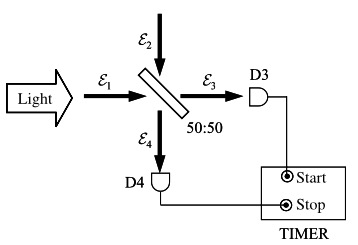
\includegraphics[width=0.5\textwidth]{figs/2022-05-09-13-44-06.png}
           \end{center}
        关心的是两个探测器测得的光强的相关性问题. 对应二阶关联函数$g^{(2)}$
   \end{frame}

   \begin{frame} 
    \frametitle{}
    \[\begin{aligned}
     g^{(2)} (t_1, t_2) &= \frac{G^{(2)}(t_1,t_2) }{[G^{(1)}(t_1) G^{(1)}(t_2)]^{1 /2} }\\ 
     &=  \frac{\left\langle a_3 ^{\dagger}(t_1)a_4^{\dagger}(t_2)a_3(t_1)a_4(t_2)  \right\rangle}{ \left\langle a_3^{\dagger}(t_1)a_3(t_1) \right\rangle  \left\langle a_4^{\dagger}(t_2)a_4(t_2) \right\rangle}  \\ 
     g^{(2)} (\tau) &= \frac{\left\langle a_3^{\dagger}(0)a_4^{\dagger}(\tau)a_3(0)a_4(\tau)  \right\rangle}{ \left\langle a_3^{\dagger}(0)a_3(0) \right\rangle  \left\langle a_4^{\dagger}(\tau)a_4(\tau) \right\rangle} \\ 
     g^{(2)} (0) &= \frac{\left\langle a_3^{\dagger}a_4^{\dagger}a_3a_4  \right\rangle}{ \left\langle a_3^{\dagger}a_3 \right\rangle  \left\langle a_4^{\dagger}a_4 \right\rangle} \\ 
    \end{aligned} \]
    下面的计算与输入的具体态相关. 
\end{frame}

\begin{frame} 
 \frametitle{}
 分束器处 in-场与out-场之间的场强关系:
 \[\begin{aligned}
    &\mathcal{E}_{3}=\left(\mathcal{E}_{1}-\mathcal{E}_{2}\right) / \sqrt{2} \\
    &\mathcal{E}_{4}=\left(\mathcal{E}_{1}+\mathcal{E}_{2}\right) / \sqrt{2}
    \end{aligned}\]
对应in-场与out-场的湮灭算符关系:
\[\begin{aligned}
    &a_{3}=\left(a_{1}-a_{2}\right) / \sqrt{2} \\
    &a_{4}=\left(a_{1}+a_{2}\right) / \sqrt{2}
    \end{aligned}\]
设1端的输入态函数为$\rs{\psi_1}$, 2端的输入态函数是真空态$\rs{0_2}$
总的输入态:
\[\rs{\Psi}= \rs{\psi_1}\rs{0_2} \]
\end{frame}

\begin{frame} 
 \frametitle{}
    \[\begin{aligned}
        \left\langle a_3^{\dagger}a_3 \right\rangle &=  \left\langle \psi_1|\ls{0_2}  a_3^{\dagger}a_3 |\rs{\psi_1}0_2\right\rangle \\ 
        &=\frac{1}{2}\left\langle \psi_1|\ls{0_2} \left(a^{\dagger}_{1}-a^{\dagger} _{2}\right)\left(a_{1}-a_{2}\right) |\rs{\psi_1}0_2\right\rangle  \\ 
        &=\frac{1}{2}\left\langle \psi_1|\ls{0_2} \left(a^{\dagger}_{1}a_{1} - a^{\dagger}_{1}a_{2} - a^{\dagger}_{2}a_{1} + a^{\dagger}_{2}a_{2} \right) \rs{\psi_1}|0_2\right\rangle  \\
        &= \frac{1}{2}\left\langle \psi_1| a^{\dagger}_{1}a_{1}  |\psi_1\right\rangle \\ 
        &= \frac{1}{2}\left\langle \psi_1| n_1 |\psi_1\right\rangle \\ 
    \left\langle a_4^{\dagger}a_4 \right\rangle &= \frac{1}{2}\left\langle \psi_1| n_1 |\psi_1\right\rangle       
    \end{aligned} \]
\end{frame}

\begin{frame} 
 \frametitle{}
 \[\begin{aligned}
    \left\langle a_3^{\dagger}a_4^{\dagger}a_3 a_4\right\rangle &= \frac{1}{4}\left\langle \Psi|(a^{\dagger} _{1}-a^{\dagger}_{2}) (a^{\dagger}_{1} + a^{\dagger}_{2})(a_{1}-a_{2})(a_{1}+a_{2})   |  \Psi \right\rangle \\ 
    &= \frac{1}{4}\left\langle \psi_1|a^{\dagger} _{1}a^{\dagger} _{1}a_{1}a_{1}   |  \psi_1 \right\rangle \\ 
    &= \frac{1}{4}\left\langle \psi_1|a^{\dagger} _{1}(a_{1}a^{\dagger} _{1} - 1)a_{1}   |  \psi_1 \right\rangle \\ 
    &= \frac{1}{4}\left\langle \psi_1| n_1(n_1-1) |  \psi_1 \right\rangle
\end{aligned} \]  
\end{frame}

\begin{frame} 
 \frametitle{}
 \[\begin{aligned}
    g^{(2)} (0) &= \frac{\left\langle a_3^{\dagger}a_4^{\dagger}a_3a_4  \right\rangle}{ \left\langle a_3^{\dagger}a_3 \right\rangle  \left\langle a_4^{\dagger}a_4 \right\rangle} \\
    &=  \frac{\frac{1}{4}\left\langle \psi_1| n_1(n_1 -1) |  \psi_1 \right\rangle}{\frac{1}{2}\left\langle \psi_1| n_1 |\psi_1\right\rangle \frac{1}{2}\left\langle \psi_1| n_1 |\psi_1\right\rangle } \\ 
    &=  \frac{\left\langle \psi_1| n_1(n_1-1) |  \psi_1 \right\rangle}{\left\langle \psi_1| n_1 |\psi_1\right\rangle^2 } \\ 
    &= \frac{\left\langle \hat{n}_1(\hat{n}_1-1)   \right\rangle}{\left\langle \hat{n}_1 \right\rangle^2 }
   \end{aligned} \] 
\end{frame}

\begin{frame} 
      \frametitle{}
    讨论:(1) 若是单光子源, 光场是$Fock$场
    \begin{enumerate}
        \item 若$\rs{\psi_1  }=\rs{0} $ \\ 
         \[g^{(2)}(0) = \frac{\left\langle 0| n_1(n_1-1) |  0 \right\rangle}{\left\langle 0| n_1 |0\right\rangle^2 } =0\]

        \item 若$\rs{\psi_1  }=\rs{n} $  \\ 
         \[g^{(2)}(0)= \frac{\left\langle n| n_1(n_1-1) |  n \right\rangle}{\left\langle n| n_1 |n \right\rangle^2 }=\frac{n(n-1)}{n^2}=1-\dfrac{1}{n}<1\]
    \end{enumerate}
   \end{frame}

   \begin{frame}
    \frametitle{}
    讨论:(2) 若是理想激光光源, 光场是相干场, 上式要对$\rs{\alpha}$态求平均. 
    \[ g^{(2)}(0) = \frac{\left\langle \alpha | a^{\dagger} _{1}a^{\dagger} _{1}a_{1}a_{1} | \alpha  \right\rangle}{ \left\langle \alpha |a^{\dagger} _{1} | \alpha\right\rangle ^2} =  \frac{\alpha^* \alpha^* \alpha \alpha }{(\alpha^* \alpha)^2 } = 1 \] 
    讨论:(3) 若是混沌光束(非理想激光光源)
    \[\begin{aligned}
        g^{(2)}(0) = \frac{\left\langle n_1(n_1-1) \right\rangle}{\left\langle n_1 \right\rangle^2 } &=\frac{\left\langle  (a^{\dagger}a)^2 \right\rangle - \left\langle a^{\dagger}a  \right\rangle}{ \left\langle  a^{\dagger} a \right\rangle ^2} \\
        &=\frac{(\Delta n)^2 + \left\langle  a^{\dagger} a \right\rangle ^2 - \left\langle a^{\dagger}a  \right\rangle}{ \left\langle  a^{\dagger} a \right\rangle ^2} \\
        &= 1 + \frac{(\Delta n)^2 - \left\langle a^{\dagger}a  \right\rangle}{ \left\langle  a^{\dagger} a \right\rangle ^2} \\ 
        &= 1 + \frac{\left\langle  a^{\dagger} a \right\rangle ^2 + \left\langle a^{\dagger}a  \right\rangle - \left\langle a^{\dagger}a  \right\rangle}{ \left\langle  a^{\dagger} a \right\rangle ^2} =2     
    \end{aligned} \]
\end{frame}

%\begin{frame} 
%      \frametitle{}
%      
%    \[\begin{aligned}
%        g^{(2)}(0)&= \frac{\left\langle a^{\dagger}a^%{\dagger}a a   \right\rangle}{ \left\langle  a^%{\dagger} a \right\rangle ^2} \\ 
%        &=\frac{\left\langle a^{\dagger}(a^{\dagger}a) %a   \right\rangle}{ \left\langle  a^{\dagger} %a \right\rangle ^2} \\
%        &=\frac{\left\langle a^{\dagger}(aa^{\dagger}%-1) a   \right\rangle}{ \left\langle  a^%{\dagger} a \right\rangle ^2} \\
%        &= \frac{\left\langle  a^{\dagger}aa^{\dagger} %a -a^{\dagger}a  \right\rangle}{ \left\langle  %a^{\dagger} a \right\rangle ^2} 
%    \end{aligned} \]
%    \end{frame}
%    
%    \begin{frame} 
%          \frametitle{}
%    \[\begin{aligned}
%        g^{(2)}(0)
%        &=\frac{\left\langle  (a^{\dagger}a)^2 %\right\rangle - \left\langle a^{\dagger}a  %\right\rangle}{ \left\langle  a^{\dagger} a %\right\rangle ^2} \\
%        &=\frac{(\Delta n)^2 + \left\langle  a^%{\dagger} a \right\rangle ^2 - \left\langle a^%{\dagger}a  \right\rangle}{ \left\langle  a^%{\dagger} a \right\rangle ^2} \\
%        &= 1 + \frac{(\Delta n)^2 - \left\langle a^%{\dagger}a  \right\rangle}{ \left\langle  a^%{\dagger} a \right\rangle ^2} \\ 
%        &= 1 + \frac{\left\langle  a^{\dagger} a %\right\rangle ^2 + \left\langle a^{\dagger}a  %\right\rangle - \left\langle a^{\dagger}a  %\right\rangle}{ \left\langle  a^{\dagger} a %\right\rangle ^2} \\
%        &=2     
%    \end{aligned} \]
%   \end{frame}

\begin{frame} 
    \frametitle{小结}
    基于二阶关联函数对光场分类:
    \begin{itemize}
        \item 反聚束光(antibunched light): $g^{(2)}(0)<1$, 非经典光, 单光子光源, 亚泊松分布 
        \item 相干光 (Coherent light) : $g^{(2)}(0)=1$, 激光, 泊松分布 (随机分布)
        \item 聚束光 (bunched light) : $g^{(2)}(0)>1$ , 经典光, 混沌光束, 过泊松分布 
    \end{itemize}
      \begin{center}
           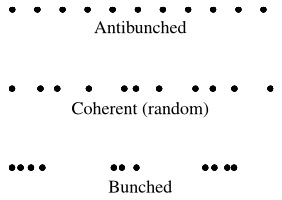
\includegraphics[width=0.4\textwidth]{figs/2022-05-09-10-30-03.png}
      \end{center}       
\end{frame}

\begin{frame}  
    \frametitle{}
    光强与光子聚束 
      \begin{center}
           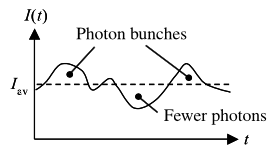
\includegraphics[width=0.5\textwidth]{figs/2022-05-09-11-42-49.png}
      \end{center}
\end{frame}

\begin{frame}  
    \frametitle{}
    二阶关联函数随时间的变化关系
      \begin{center}
           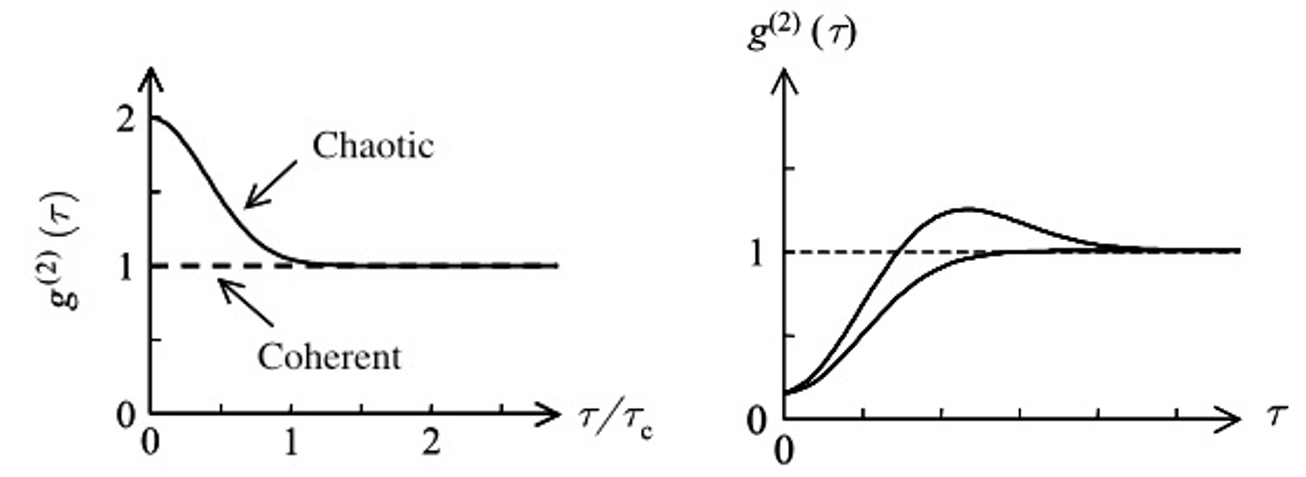
\includegraphics[width=0.8\textwidth]{figs/21.png}
      \end{center}
\end{frame}

\begin{frame} 
    \frametitle{反聚束光实验制备}
    ~ \\
    \begin{enumerate}
        \item 单原子
        \item 掺杂在晶体中的荧光染料分子
        \item 半导体量子点
        \item 金刚石色心
    \end{enumerate}
          \begin{center}
               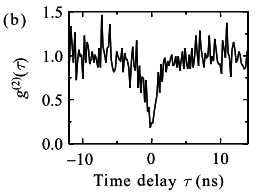
\includegraphics[width=0.43\textwidth]{figs/2022-05-09-12-08-59.png}
          \end{center}
\end{frame}

\begin{frame} 
\frametitle{HB-T 星光测量}
     \[ \begin{aligned}
        G^{(2)}&(x_1, x_2; x_3,x_4) = \left\langle E^{(-)}(x_1)E^{(-)}(x_2)E^{(+)}(x_3)E^{(+)}(x_4) \right\rangle \\
        &= \left\langle 1_k, 1_{k'} \left| E^{(-)}(x_1)E^{(-)}(x_2)E^{(+)}(x_3)E^{(+)}(x_4) \right| 1_{k'}, 1_k \right\rangle \\
        &= \sum_{\{ n\}} \left\langle 1_k, 1_{k'} \left| E^{(-)}(x_1)E^{(-)}(x_2)  \left| \{ n\} \left\rangle  \right\langle \{ n\} \right| E^{(+)}(x_3)E^{(+)}(x_4) \right| 1_{k'}, 1_k \right\rangle \\
        &= \left\langle 1_k, 1_{k'} \left| E^{(-)}(x_1)E^{(-)}(x_2)  \left| 0 \left\rangle  \right\langle 0 \right| E^{(+)}(x_3)E^{(+)}(x_4) \right| 1_{k'}, 1_k \right\rangle \\ 
        &= \left\langle 0 \left| E^{(+)}(x_1)E^{(+)}(x_2)  \left| 1_k, 1_{k'}  \left\rangle^*  \right\langle 0 \right| E^{(+)}(x_3)E^{(+)}(x_4) \right| 1_{k'}, 1_k \right\rangle
     \end{aligned}\] 
    代入:
    \[\hat{E}^{(+)} (x_i) + \hat{E}^{(-)}(x_i) =\epsilon_k a_k e^{-i(v_k t - \mathbf{k}\cdot \mathbf{r}_i)} + \epsilon_k a^{\dagger} _k e^{i(v_k t - \mathbf{k}\cdot \mathbf{r}_i)}\]
    进行计算, 并令 $x_{1}=x_3, x_2=x_4$, 可得: 
    \[ G^{(2)} = 2 \left|\epsilon_k\right|^4 \left\{ 1+ \cos (\mathbf{k} - \mathbf{k}')\cdot (\mathbf{r}- \mathbf{r}')  \right\}\]
\end{frame}


\begin{frame} 
\frametitle{}
     分析: \\ 
     \[ G^{(2)} = 2 \left|\epsilon_k\right|^4 \left\{ 1+ \cos (\mathbf{k} - \mathbf{k}')\cdot (\mathbf{r}- \mathbf{r}')  \right\}\]
     (1) 干涉项源于夹角(对应恒星直径) \\ 
     \[\cos (\mathbf{k} - \mathbf{k}')\cdot (\mathbf{r}- \mathbf{r}') \]
     (2) 公式中没有敏感项
     \[ \cos\left[ (\mathbf{k} + \mathbf{k}') \cdot \mathbf{r}_0 \right] \]
     因此可以测得更大更远的恒星星光 \\ 
     (3) 公式可写成平均粒子数形式(设两光束光强相同)
     \[ G^{(2)} = 2 \left|\epsilon_k\right|^4 \left\{ \left|n^2\right| - \left|n\right|+ \left| n \right|^2\cos (\mathbf{k} - \mathbf{k}')\cdot (\mathbf{r}- \mathbf{r}')  \right\}\]
     光强关联的本质在于光子数均值及涨落的关联 \\
     (4) 所有的HB-T测量都是基于二阶关联函数的测量
\end{frame}

\begin{frame} 
\frametitle{}
     (5) 对于两电子(费米子), 其反对易关系导致二阶关联函数取如下形式:
     \[ G^{(2)} = 2 \left|\epsilon_k\right|^4 \left\{ 1- \cos (\mathbf{k} - \mathbf{k}')\cdot (\mathbf{r}- \mathbf{r}')  \right\}\]
     两电子之间也存在二阶关联.
\end{frame}
%%%%%%%%%%%%%%%%%%%%%%%%%%%%%%%%%%%%%%%%%%%%%%%%%%%%%%%%%%%%%%%%%%%
\begin{frame} 
    \frametitle{课外作业}
    对于热辐射场, 混沌光束, 激光, 压缩光, Fock光, 真空态
    \begin{enumerate}
        \item 写出 $\overline{n}$ 和 $\overline{n^2}$
        \item 写出分布函数 $P(n)$
        \item 写出二阶关联函数 $g^{(2)}(0)$
    \end{enumerate}
\end{frame}
%%%%%%%%%%%%%%%%%%%%%%%%%%%%%%%%%%%%%%%%%%%%%%%%%%%%%%%%%%%%%%%%%%%